\subsubsection{bringit::client::usecase::ForwardListUseCase}

\label{bringit::client::usecase::ForwardListUseCase}
\begin{figure}[H]
	\centering
	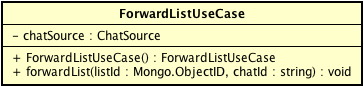
\includegraphics[scale=0.5]{Sezioni/SottosezioniST/img/app/ForwardListUseCase.png}
	\caption{bringit::client::usecase::ForwardListUseCase}
\end{figure}

\begin{itemize}
\item \textbf{Descrizione}: Questa classe rappresenta l'inoltro di liste bringit nella chat di Rocket.Chat.
\item \textbf{Utilizzo}: La classe viene utilizzata per l'inoltro di liste bringit nei vari canali di chat di Rocket.Chat.
\item \textbf{Attributi}: 
	\begin{itemize}
	\item \textit{private chatSource:ChatSource}\\
	L'oggetto ChatSource per interfacciarsi alla chat di Rocket.Chat.
	\end{itemize}
\item \textbf{Metodi}:
	\begin{itemize}
	\item \textit{public ForwardListUseCase():ForwardListUseCase}\\
	Il costruttore della classe ForwardListUseCase.
	\item \textit{public forwardList(listId:string,roomName:string):void}\\
	Questo metodo inoltra una lista bringit in un canale di Rocket.Chat.
			\\ \textbf{Parametri}: \begin{itemize}
				\item \textit{listId:string}\\
				L'identificativo della lista che si vuole inoltrare.
				\item \textit{roomName:string}\\
				Il canale \termine{Rocket.Chat} nel quale si vuole inoltrare la lista.
			\end{itemize}
	\end{itemize}
\end{itemize} 

\subsubsection{bringit::client::usecase::ShowPopupUseCase}

\label{bringit::client::usecase::ShowPopupUseCase}
\begin{figure}[H]
	\centering
	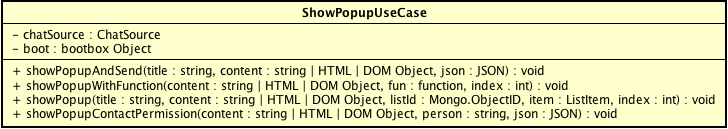
\includegraphics[scale=0.5]{Sezioni/SottosezioniST/img/app/ShowPopupUseCase.png}
	\caption{bringit::client::usecase::ShowPopupUseCase}
\end{figure}

\begin{itemize}
\item \textbf{Descrizione}: Questa classe rappresenta la visualizzazione di popup nella chat di Rocket.Chat.
\item \textbf{Utilizzo}: La classe viene utilizzata per la visualizzazione di popup nei vari canali di chat di Rocket.Chat.
\item \textbf{Attributi}: 
	\begin{itemize}
	\item \textit{private chatSource:ChatSource}\\
	L'oggetto ChatSource per interfacciarsi alla chat di Rocket.Chat.
	\item \textit{private boot:Object}\\
	Questo attributo è necessario per l'utilizzo della libreria bootbox, che viene usata per la visualizzazione dei popup in Bringit.
	\end{itemize}
\item \textbf{Metodi}:
	\begin{itemize}
	\item \textit{public ShowPopupUseCase():ShowPopupUseCase}\\
	Il costruttore della classe ShowPopupUseCase.
	\item \textit{public showPopupAndSend(title:string,content:string,json:JSONObject):void}\\
	Questo metodo visualizza un popup in \termine{Rocket.Chat} e inoltra un messaggio.
			\\ \textbf{Parametri}: \begin{itemize}
				\item \textit{title:string}\\
				Il titolo del popup.
				\item \textit{content:string}\\
				Il contenuto del popup.
				\item \textit{json:JSONObject}\\
				Il messaggio che verrà mandato dopo la visualizzazione del popup.
			\end{itemize}
	\item \textit{public showPopupWithFunction(content, fun, index:number):void}\\
	Questo metodo visualizza un popup in \termine{Rocket.Chat} e esegue una funzione una volta chiuso.
			\\ \textbf{Parametri}: \begin{itemize}
				\item \textit{content:string}\\
				Il contenuto del popup.
				\item \textit{fun:function}\\
				La funzione da eseguire alla chiusura del popup.
				\item \textit{index:number}\\
				Questo parametro viene utilizzato per la scelta del tipo di modale.
			\end{itemize}
	\item \textit{public showPopupContactPermission(content:string,person:string,json:JSONObject):void}\\
	Questo metodo visualizza un popup in \termine{Rocket.Chat} e esegue una funzione in maniera asincrona una volta chiuso. Questo metodo è usato per la concessione di permessi a un altro utente.
			\\ \textbf{Parametri}: \begin{itemize}
				\item \textit{content:string}\\
				Il contenuto del popup che sarà mostrato.
				\item \textit{person:string}\\
				La persona alla quale vengono concessi i permessi.
				\item \textit{json:JSONObject}\\
				Il messaggio che è stato mandato.
			\end{itemize}
	\end{itemize}
\end{itemize}